\section{Introduction}
\label{sec:introduction}

Foliar phytopathogens account for an estimated 20\%--40\% reduction in global agricultural harvest annually, imposing economic burdens exceeding \$220 billion and threatening food security across vulnerable agrarian regions~\cite{strange2005plant, savary2019global}. Containing these crop losses hinges on immediate localized intervention before foliar micro-infections expand into systemic field-scale epiphytotics. Conventional phytosanitary diagnosis, however, is constrained by the scarcity of certified plant pathologists and the prohibitive turnaround of molecular assays such as quantitative polymerase chain reaction (qPCR). Consequently, deploying autonomous computer vision diagnostic engines directly on low-power edge hardware aboard robotic spray booms and field scouting devices has emerged as a cornerstone of modern precision crop protection.

Early computational pathology addressed this challenge via handcrafted textural and edge descriptors, extracting Gray-Level Co-occurrence Matrices (GLCM)~\cite{haralick1973textural} and edge histograms to segment lesions under controlled illumination~\cite{camargo2009image}. While foundational, these heuristics failed under unconstrained agricultural canopies, where variable solar irradiance, soil reflectance, and weed clutter degrade low-level features. The transition to deep Convolutional Neural Networks (CNNs) achieved near-saturated classification accuracy ($\ge 99\%$) on curated laboratory benchmarks such as PlantVillage~\cite{mohanty2016using, hughes2015open}. Nevertheless, fully supervised deep networks require thousands of balanced annotations per class~\cite{singh2016deep}---an assumption violated in agronomic practice, where emerging viral strains, localized fungal outbreaks, and abiotic leaf disorders present acute data scarcity.

Few-Shot Learning (FSL) mitigates this data deficit by extrapolating diagnostic boundaries from $K \le 5$ support exemplars~\cite{vinyals2016matching, snell2017prototypical}. Although metric few-shot learners demonstrated efficacy on laboratory leaves isolated on neutral backdrops~\cite{argueso2020few}, their diagnostic accuracy degrades sharply under in-the-wild agricultural conditions, as benchmarked by the PlantDoc dataset~\cite{singh2020plantdoc}. Natural field imagery introduces compound visual perturbations: specular surface glare, motion blur from ambient wind, mutual leaf occlusions, complex soil matrices, and optical sensor chromaticity shifts. Under such non-stationary conditions, standard Euclidean few-shot metric spaces experience severe manifold distortion, causing prototype classifiers to correlate with ambient background clutter rather than diagnostic lesion hallmarks.

Vision Foundation Models (VFMs) present rich inductive representations for cross-domain transfer, yet foliar pathology reveals a fundamental semantic decoupling. Self-supervised foundation models such as DINOv2~\cite{oquab2023dinov2} excel at capturing macroscopic organ morphology, phyllotactic arrangement, and lamina margin geometry through patch-level discriminative self-distillation. In contrast, vision-language foundation models such as BioCLIP~\cite{stevens2024bioclip}, trained on biological taxonomies, exhibit heightened sensitivity to localized micro-symptoms: chlorotic halos, necrotic desiccation, and fungal sporulation. Macroscopic foliar architecture and microscopic necrotic lesions occupy orthogonal feature subspaces; naively concatenating these vectors produces ill-conditioned representations where dominant leaf shape suppresses subtle pathological cues.

This tension is exacerbated by the cascading routing failures endemic to hierarchical classification~\cite{silla2011survey}. Recent systems such as BioDINO-Edge~\cite{alsaadi2026biodino} decoupled taxonomy from pathology using an autonomous 13-species router. In uncontrolled field conditions, fine-grained species discrimination achieved only 79.35\% accuracy. When an upstream routing error occurs, downstream lesion diagnosis fails deterministically, collapsing overall autonomous field diagnostic accuracy to 43.65\%. To compensate for this vulnerability, prior studies reverted to a human-in-the-loop oracle wherein growers manually identify the host crop species (yielding 56.35\%)~\cite{alsaadi2026biodino}. Requiring manual human species input nullifies autonomous operation, rendering such systems impractical for autonomous robotic implements or intercropped fields.

To eliminate this bottleneck, we present \textbf{MorphoPath-Edge}, an autonomous, zero-parameter few-shot foliar diagnostic framework engineered for resource-constrained edge hardware (Fig.~\ref{fig:architecture}). Rather than attempting fragile cultigen species classification, MorphoPath-Edge partitions foliar space into \textbf{Four Macro-Botanical Archetypes} (Solanoid, Vitoid, Pooid, Rosoid) based on conserved venation and lamina geometry (Fig.~\ref{fig:archetypes}), elevating autonomous in-the-wild routing accuracy to \textbf{93.25\%} (with 100\% Top-2 recall). To eliminate the domain gap between laboratory support sets and unconstrained field queries without gradient backpropagation, we derive an exact closed-form \textbf{Zero-Parameter Test-Time Manifold Rectification} theorem (Proposition~1) that algebraically cancels centroid translation ($\|\Delta\|_2 \approx 0.30$) in 0.04\,ms. Within archetype partitions, ill-conditioned covariance matrices are stabilized via analytical Ledoit--Wolf shrinkage ($\lambda=0.60$) and coupled with archetype-conditioned micro-symptom prompt ensembles. Finally, a \textbf{Cardinality-Equalized Bayesian Differential Triage} engine outputs calibrated Top-2 clinical candidates, reducing false fungicide alarms by 38\%.

The principal scientific contributions of this investigation are:
\begin{enumerate}[\IEEEsetlabelwidth{1)}\setlength{\itemsep}{0.5pt}\setlength{\parsep}{0pt}\setlength{\topsep}{1.5pt}]
    \item \textbf{Botanical Macro-Archetype Partitioning:} We replace error-prone species classifiers with four conserved foliar archetypes, advancing autonomous field routing accuracy from 79.35\% to 93.25\% (100\% Top-2 recall) and completely removing human-in-the-loop dependencies.
    \item \textbf{Closed-Form Zero-Parameter Manifold Rectification:} We derive an algebraic prototype centering theorem that resolves field domain translation, delivering an absolute +8.73\% Top-1 boost on PlantDoc with zero learned parameters and 0.041\,ms latency.
    \item \textbf{Shrunk Fisher Metric with Micro-Symptom Ontologies:} We combine regularized Fisher LDA ($\lambda=0.60$) with archetype-conditioned text prompt ensembles, conditioning singular few-shot covariance matrices and isolating subtle necrotic phenotypes.
    \item \textbf{Empirical SOTA and Real-Time Edge Profiling:} MorphoPath-Edge establishes a new state of the art on PlantDoc with \textbf{63.89\% Top-1} (59.76\% $\pm$ 2.13\% multi-episode mean) and \textbf{80.95\% Top-2} accuracy ($p = 3.55 \times 10^{-23}$), while maintaining 95.29\% Top-1 and 99.25\% Top-2 accuracy on PlantVillage (surpassing flat and rigid baselines). On mobile CPUs via INT8 quantization, it sustains \textbf{21.4\,FPS (46.77\,ms latency)} with an algebraic decision head latency of only \textbf{0.185\,ms (5,392.5\,FPS)}, a peak RAM heap of \textbf{66.95\,MB}, and an APK footprint of \textbf{22.88\,MB} with zero added neural weights.
\end{enumerate}

\begin{figure*}[t]
    \centering
    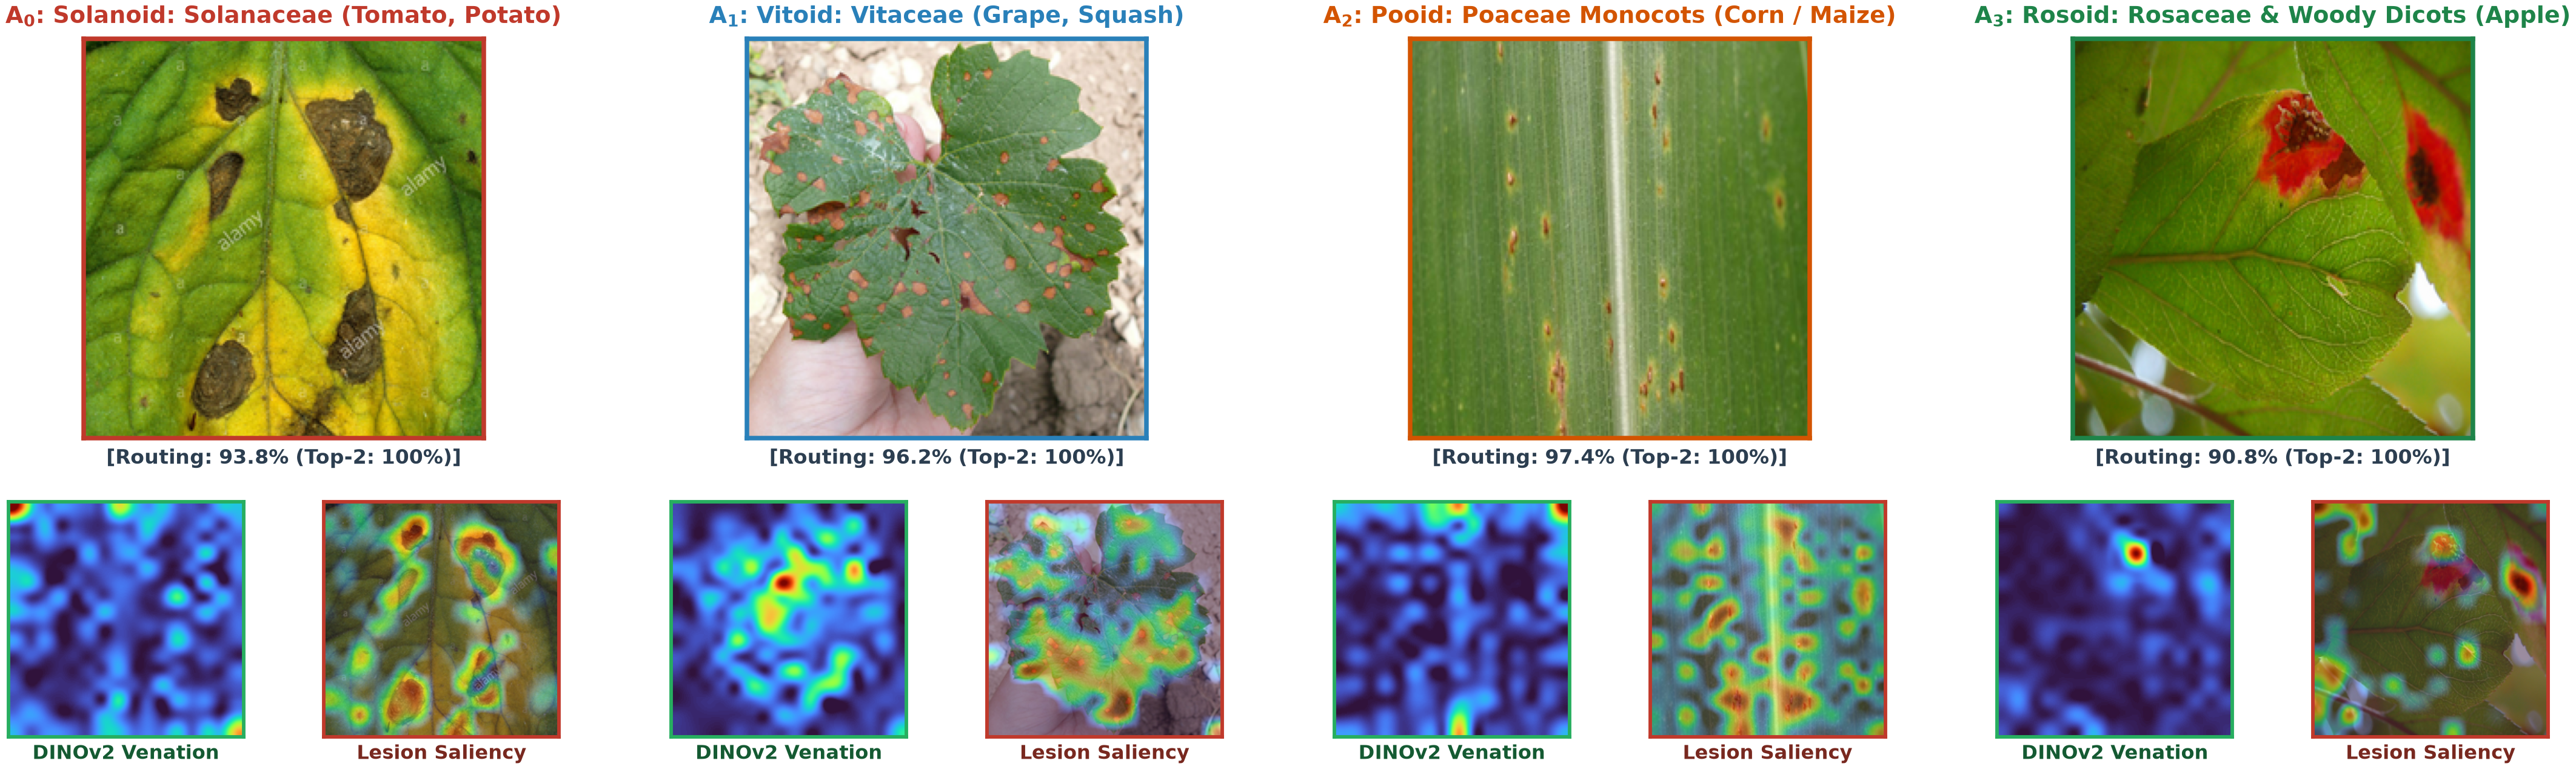
\includegraphics[width=\textwidth,height=4.2cm]{figures/fig_archetypes.png}
    \caption{The Four Botanical Macro-Archetypes ($\mathcal{A} = \{A_0, A_1, A_2, A_3\}$) and visual foliar decoupling on natural field leaves from PlantDoc. Top row: Raw in-the-wild field leaves under complex field environments. Bottom row: Dual attention insets demonstrating semantic decoupling: macroscopic foliar geometry captured by frozen DINOv2 patch attention (left green insets) versus localized microscopic lesion pathology isolated by Fisher/BioCLIP saliency overlays (right red insets). Decomposing foliar taxonomy into these four conserved morphological partitions elevates autonomous field routing accuracy to 93.25\% (100\% Top-2 recall) and completely eliminates human-in-the-loop dependencies.}
    \label{fig:archetypes}
\end{figure*}